\newpage
\section{正交曲线坐标系}
\subsection{常用的正交曲线坐标系}
正交曲线坐标系:空间任意一点,所有坐标线相互垂直
$$\begin{aligned}
\text{极坐标系:}\\
x=&r\cos\phi\\
y=&r\sin\phi
\end{aligned}
\quad
\begin{aligned}
\text{柱坐标系:}\\
x=&r\cos\phi\\
y=&r\sin\phi\\
z=&z
\end{aligned}
\quad
\begin{aligned}
\text{球坐标系:}\\
x=&r\sin\theta\cos\phi\\
y=&r\sin\theta\sin\phi\\
z=&r\cos\theta
\end{aligned}
\begin{aligned}
    \text{抛物坐标系:}\\
    x=&\sqrt{\xi\eta}\cos\phi\\
    y=&\sqrt{\xi\eta}\sin\phi\\
    z=&\frac{1}{2}(\xi-\eta)
\end{aligned}
$$

\begin{figure}[H]
    \centering 
    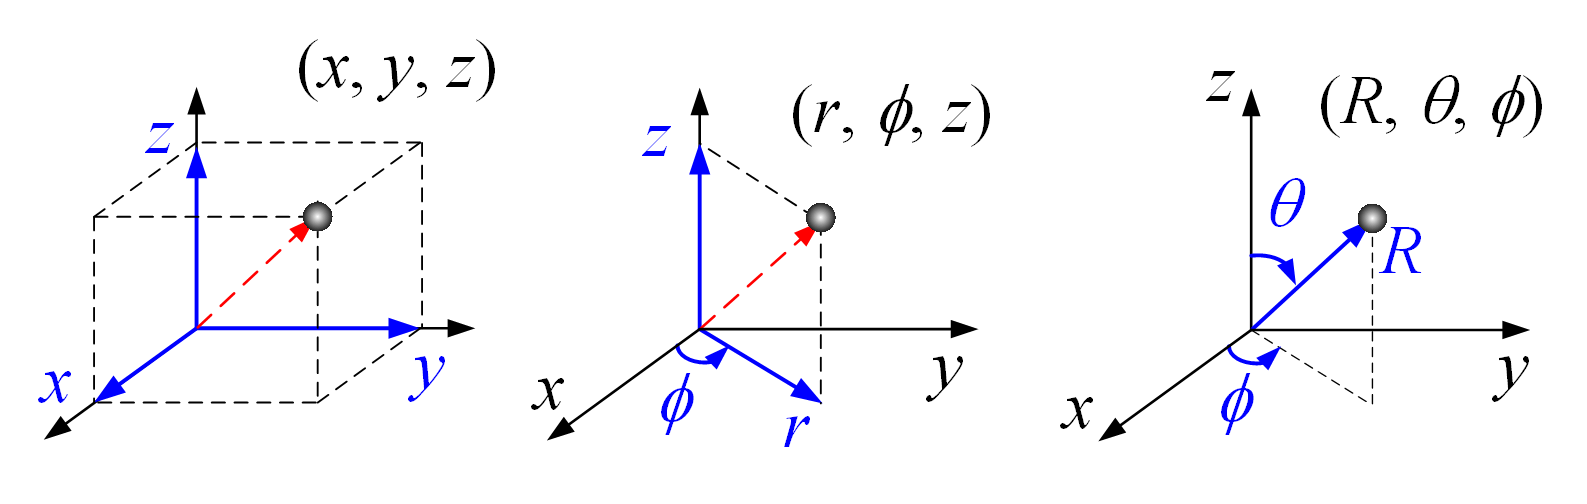
\includegraphics[width=13cm]{figures/3Coordinates.png} 
    \caption{直角坐标系,柱坐标与球坐标} 
    \label{3Coordinates}
\end{figure}

\subsection{正交曲线坐标的判别法:度规法}
曲线坐标系$(x_1,x_2,x_3)$,$x=x(x_1,x_2,x_3),y=y(y_1,y_2,y_3),z=x(x_1,x_2,x_3)$
$$\begin{aligned}
    dx=&\frac{\partial x}{\partial x_1}dx_1+\frac{\partial x}{\partial x_2}dx_2+\frac{\partial x}{\partial x_3}dx_3\\
    dy=&\frac{\partial y}{\partial x_1}dx_1+\frac{\partial y}{\partial x_2}dx_2+\frac{\partial y}{\partial x_3}dx_3\\
    dz=&\frac{\partial z}{\partial x_1}dx_1+\frac{\partial z}{\partial x_2}dx_2+\frac{\partial z}{\partial x_3}dx_3
\end{aligned}$$

距离微元
$$\begin{aligned}
    ds^2\equiv&dx^2+dy^2+dz^2\\
    =&\left(\frac{\partial x}{\partial x_1}dx_1+\frac{\partial x}{\partial x_2}dx_2+\frac{\partial x}{\partial x_3}dx_3\right)^2+\left(\frac{\partial y}{\partial x_1}dx_1+\frac{\partial y}{\partial x_2}dx_2+\frac{\partial y}{\partial x_3}dx_3\right)^2\\
    &+\left(\frac{\partial z}{\partial x_1}dx_1+\frac{\partial z}{\partial x_2}dx_2+\frac{\partial z}{\partial x_3}dx_3\right)^2\\
    =&\sum_{i,j=1,2,3}g_{ij}dx_idx_j\\
    \equiv&g_{11}(dx_1)^2+g_{22}(dx_2)^2+g_{33}(dx_3)^2+2g_{12}dx_1dx_2+2g_{13}dx_1dx_3+2g_{23}dx_2dx_3
\end{aligned}$$
其中,
$$g_{ij}=g_{ji}=\frac{\partial x}{\partial x_i}\frac{\partial x}{\partial x_j}+\frac{\partial y}{\partial x_i}\frac{\partial y}{\partial x_j}+\frac{\partial z}{\partial x_i}\frac{\partial z}{\partial x_j}$$
柱坐标:$$ds^2=[d(r\cos\phi)]^2+[d(r\sin\phi)]^2+dz^2=dr^2+r^2d\phi^2+dz^2$$
球坐标:$$ds^2=dr^2+r^2d\theta^2+r^2\sin^2\theta d\phi^2$$
抛物坐标:$$ds^2=\frac{\xi+\eta}{4\xi}(d\xi)^2+\frac{\xi+\eta}{4\eta}(d\eta)^2+\xi\eta(d\phi)^2$$
\begin{thm}[度规法]
    $ds^2$\textbf{无交叉项}$\Leftrightarrow$正交曲线坐标系
$$ds^2=(h_1dx_1)^2+(h_2dx_2)^2+(h_3dx_3)^2$$
其中,
$$g_{11}=h_1^2,g_{22}=h_2^2,g_{33}=h_3^2$$
\end{thm}



\subsection{正交曲线坐标的微分算子}
梯度$\nabla u$
$$\nabla u=\frac{1}{h_1 }\frac{\partial u}{\partial x_1}\vec{e}_1+\frac{1}{h_2 }\frac{\partial u}{\partial x_2}\vec{e}_2+\frac{1}{h_3 }\frac{\partial u}{\partial x_3}\vec{e}_3$$

散度$\nabla\cdot\vec{v}$
$$\begin{aligned}
    \nabla\cdot\vec v=&\frac{\mbox{净通量}}{h_1h_2h_3dx_1dx_2dx_3}\\=&\frac{1}{h_1h_2h_3}\left[\frac{\partial}{\partial x_1}(v_1h_2h_3)+\frac{\partial}{\partial x_2}(v_2h_1h_3)+\frac{\partial}{\partial x_3}(v_3h_1h_2)\right]
    \end{aligned}$$

Laplacian $\nabla^2u=\nabla\cdot(\nabla u)$
$$
\nabla^2u=\frac{1}{h_1h_2h_3}\left[\frac{\partial}{\partial x_1}\left(\frac{h_2h_3}{h_1}\frac{\partial u}{\partial x_1}\right)+\frac{\partial}{\partial x_2}\left(\frac{h_1h_3}{h_2}\frac{\partial u}{\partial x_2}\right)+\frac{\partial}{\partial x_3}\left(\frac{h_1h_2}{h_3}\frac{\partial u}{\partial x_3}\right)\right]
$$

$$\begin{aligned}
\text{柱坐标}\quad&\nabla^2u=\frac{1}{r}\frac{\partial}{\partial r}\left(r\frac{\partial u}{\partial r}\right)+\frac{1}{r^2}\frac{\partial^2u}{\partial \phi^2}+\frac{\partial^2 u}{\partial z^2}\\
\text{球坐标}\quad&\nabla^2u=\frac{1}{r^2}\frac{\partial}{\partial r}
\left(r^2\frac{\partial u}{\partial r}\right)+\frac{1}{r^2\sin\theta}\frac{\partial}{\partial\theta}
\left(\sin\theta\frac{\partial u}{\partial \theta}\right)+\frac{1}{r^2\sin^2\theta}\frac{\partial^2 u}{\partial \phi^2}
\end{aligned}$$



\subsection{正交曲线坐标的分离变量}
\begin{ex}[极坐标下的稳态传热问题]
    $$\left\{
        \begin{aligned}
        &
        \frac{1}{r}\frac{\partial}{\partial r}\left(r\frac{\partial u}{\partial r}\right)+\frac{1}{r^2}\frac{\partial^2u}{\partial\phi^2}=0,0<r<a,0<\phi<2\pi\\
        &u|_{r=a}=f(\phi)\\
        &u|_{\phi=0}=u|_{\phi=2\pi},\frac{\partial u}{\partial \phi}\bigg|_{\phi=0}=\frac{\partial u}{\partial \phi}\bigg|_{\phi=2\pi}\\
        &u|_{r=0}<\infty
                \end{aligned}
        \right.$$
    
        \textbf{1. 分离变量}

        设$u=R(r)\Phi(\phi)$
        $$\Rightarrow\left\{
    \begin{aligned}
    &
    \frac{1}{r}\frac{d}{d r}\left(r\frac{dR}{dr}\right)-\lambda R=0\\
    &R(0)<\infty
            \end{aligned}
    \right.
    \quad
    \left\{
    \begin{aligned}
    &
    \Phi''(\phi)+\lambda\Phi(\phi)=0 \\
    &\Phi(0)=\Phi(2\pi),\Phi'(0)=\Phi'(2\pi)
            \end{aligned}
    \right.$$

    \textbf{2. 本征值问题}

    $$\begin{aligned}
        \mathrm{i}. &\lambda=0\Rightarrow \Phi_0(0)=1\\
        \mathrm{ii}. &\lambda<0\mbox{,无解}\\
        \mathrm{iii}. &\lambda>0\Rightarrow\Phi=A\sin\sqrt\lambda\phi+B\cos\sqrt\lambda\phi
    \end{aligned}$$
    $$\begin{aligned}
        \Phi(0)&=\Phi(2\pi)\Rightarrow B=A\sin(2\pi\sqrt\lambda)+B\cos(2\pi\sqrt\lambda)\\
        \Phi'(0)&=\Phi'(2\pi)\Rightarrow A=A\cos(2\pi\sqrt\lambda)-B\sin(2\pi\sqrt\lambda)
    \end{aligned}$$
    $$\left | \begin{matrix}
        \sin(2\pi\sqrt\lambda) &\cos(2\pi\sqrt\lambda)-1\\
        \cos(2\pi\sqrt\lambda)-1 &-\sin(2\pi\sqrt\lambda) \\
        \end{matrix} \right | =0\Rightarrow\cos(2\pi\sqrt\lambda)=1$$

    本征值:$\lambda_m=m^2,m=1,2,...,A,B$任意

    本征函数:$\Phi_{m1}=\sin{m\phi},\Phi_{m2}=\cos{m\phi}$

    \textbf{3. 乘积型解}
    $$r\frac{d}{d r}\left(r\frac{dR}{dr}\right)-\lambda R=0$$

    即欧拉方程,采用变量代换:
    $$r=e^t\quad,\frac{d}{dt}=\frac{dr}{dt}\frac{d}{dr}=r\frac{d}{dr}$$

    得到关于$t$的ODE
    $$\frac{d^2R(t)}{dt^2}-\lambda R(t)=0$$

    i. $\lambda=0\Rightarrow R_0(t)=C_0+D_0t=C_0+D_0\ln r$

    ii. $\lambda_m=m^2,m=1,2,3,...$
      $$R_m=C_me^{mt}+D_me^{-mt}=C_mr^m+D_mr^{-m}$$
    $$u(r,\phi)=C_0+\sum_{m=1}^\infty \left(C_{m1}r^m\sin{m\phi}+C_{m2}r^m\cos{m\phi}\right)$$

    (由于$u|_{r=0}<\infty,$没有$D_{m}r^{-m}$和$D_0\ln r$项)
    $$u|_{r=a}=f(\phi)=C_0+\sum_{m=1}^\infty a^m\left(C_{m1}\sin{m\phi}+C_{m2}\cos{m\phi}\right)$$

    \textbf{4. 完整解}
    $$\begin{aligned}
    C_0=&\frac{1}{2\pi}\int_0^{2\pi}f(\phi)d\phi\\
    C_{m1}=&\frac{1}{\pi  a^m}\int_0^{2\pi}f(\phi)\sin(m\phi)d\phi\\
    C_{m2}=&\frac{1}{\pi  a^m}\int_0^{2\pi}f(\phi)\cos(m\phi)d\phi
    \end{aligned}$$
    $$u(r,\phi)=C_0+\sum_{m=1}^\infty r^m\left(C_{m1}\sin{m\phi}+C_{m2}\cos{m\phi}\right)$$
\end{ex}
